\documentclass{beamer}
\usepackage{booktabs}
\usepackage{amsmath}
\usepackage{blkarray}
\usepackage{tikz}
\usepackage{subfigure}

\usepackage{pdfpages}
%\pdfpagelayout{2 on 1}[letterpaper,border shrink=5mm]

\mode<presentation>
{
%  \usetheme{Malmoe}
  \usetheme{default}
  %\usecolortheme{seahorse}
  % or ...

 \setbeamercovered{transparent}
  % or whatever (possibly just delete it)
 \setbeamertemplate{footline}[default]
 \setbeamertemplate{navigation symbols}{\insertslidenavigationsymbol\insertframenavigationsymbol\insertdocnavigationsymbol}
}


\usepackage[english]{babel}
% or whatever

%\usepackage[latin1]{inputenc}
% or whatever

%\usepackage{times}
%\usepackage[T1,T5]{fontenc}
% Or whatever. Note that the encoding and the font should match. If T1
% does not look nice, try deleting the line with the fontenc.

\def\showlogo{%
  \begin{tikzpicture}[remember picture,overlay]
    \node[anchor=north east,yshift=1pt] at (current page.north east) {
      
\includegraphics[height=.6cm,width=2.5cm]{ncats-logo}
    };
  \end{tikzpicture}
}

\def\showlogoSW{%
  \begin{tikzpicture}[remember picture,overlay]
    \node[anchor=south west,yshift=1pt] at (current page.south west) {
      
\includegraphics[height=.6cm,width=2.5cm]{ncats-logo}
    };
  \end{tikzpicture}  
}  

\title{Do Structurally Similar InChIs\\ Have Similar Hash Keys?}

%\subtitle{Include Only If Paper Has a Subtitle}

\author{Dac-Trung Nguyen}
% - Give the names in the same order as the appear in the paper.
% - Use the \inst{?} command only if the authors have different
%   affiliation.

\institute[NCATS] % (optional, but mostly needed)
          {National Center for Advancing Translational Sciences\\
            National Institutes of Health}
%\href{https://ncats.nih.gov}{\texttt{https://ncats.nih.gov}}}
% - Use the \inst command only if there are several affiliations.
% - Keep it simple, no one is interested in your street address.

\date[]% (optional, should be abbreviation of conference name)
{InChI Virtual Workshop\\ March 22--24, 2021}
% - Either use conference name or its abbreviation.
% - Not really informative to the audience, more for people (including
%   yourself) who are reading the slides online

%\subject{Theoretical Computer Science}
% This is only inserted into the PDF information catalog. Can be left
% out. 


% If you have a file called "university-logo-filename.xxx", where xxx
% is a graphic format that can be processed by latex or pdflatex,
% resp., then you can add a logo as follows:

%\pgfdeclareimage[height=.6cm,width=2.5cm]{ncats-logo}{ncats-logo}
%\logo{\pgfuseimage{ncats-logo}}

% Delete this, if you do not want the table of contents to pop up at
% the beginning of each subsection:
%\AtBeginSubsection[]
%{
%  \begin{frame}<beamer>
%    \frametitle{Outline}
%    \tableofcontents[currentsection,currentsubsection]
%  \end{frame}
%}


% If you wish to uncover everything in a step-wise fashion, uncomment
% the following command: 

%\beamerdefaultoverlayspecification{<+->}


\begin{document}

\begin{frame}
  \showlogoSW  
  \titlepage
\end{frame}

%\addtobeamertemplate{frametitle}{}{\showlogo}

\begin{frame}
  \showlogoSW
  \begin{quote}
    InChI is the greatest thing ever since sliced ​​bread.
    \begin{flushright}
      \tiny{---Steve Heller}
    \end{flushright}
  \end{quote}
  \begin{quote}
    InChIKey is perhaps the greatest thing ever since butter.
    \begin{flushright}
      \tiny{---Dac-Trung Nguyen}
    \end{flushright}
  \end{quote}
  InChIKey is a hash key with...
  \begin{enumerate}[(i)]
  \item Compact representation (27 characters)
  \item Structural ``hints'' (\texttt{UHFFFAOYSA} and charge suffix \texttt{-N})
    \begin{itemize}
      % 81386624 / 109803102 as of mar 17, 2021
      \item Approximately 74\% of structures in PubChem contains \texttt{UHFFFAOYSA}
    \end{itemize}
  \item Collision resistance (truncated SHA-2 with very low probability of collision)
  \end{enumerate}
  InChIKey is well-suited for applications that require uniqueness (e.g., resolver). However, for many use cases such as registration and HTS analysis, we would like a more flexible hash key that can facilitate ``meaningful'' comparison while retaining relevant features of InChIKey. This is the story of \emph{\color{blue}{spectral hash key}} for InChI.

\end{frame}

\begin{frame}
  \showlogo
  \frametitle{Spectral hash key at a glance}
  \begin{columns}
    \column{3cm}
    \texttt{CHEMBL279476}\\ \vspace{1em}
    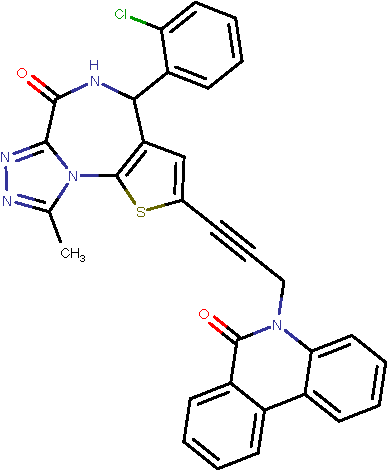
\includegraphics[width=3cm]{CHEMBL279476-crop}
    \vtop{%
      \begin{tiny}
        \hbox{\texttt{PVSICLYUDGZPCO-UHFFFAOYSA-N}}
\hbox{\texttt{\color{red}{111ZMSDKX}\color{blue}{4LX8LNL6ZR}\color{black}{D728VM5HM7J}}}
      \end{tiny}
    }
    \column{3cm}
    \texttt{CHEMBL282495}\\ \vspace{1em}
    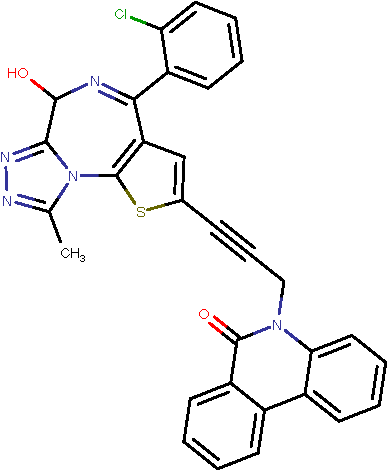
\includegraphics[width=3cm]{CHEMBL282495-crop}
    \vtop{%
      \begin{tiny}
        \hbox{\texttt{GTTQCZXVNFENHV-UHFFFAOYSA-N}}
\hbox{\texttt{\color{red}{111ZMSDKX}\color{blue}{4LX8LNL6ZR}\color{black}{UL5DJK5J2XW}}}
      \end{tiny}
    }    
    \column{3cm}
    \texttt{CHEMBL20178}\\ \vspace{1em}
    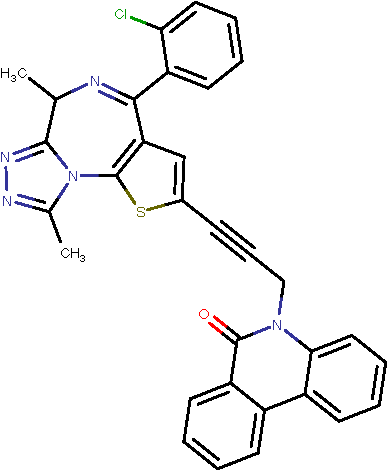
\includegraphics[width=3cm]{CHEMBL20178-crop}
    \vtop{%
      \begin{tiny}
        \hbox{\texttt{ZIJDJRBEHTWHFS-UHFFFAOYSA-N}}
\hbox{\texttt{\color{red}{111ZMSDKX}\color{black}{W278SN92KHW12FPL5V1YL}}}
      \end{tiny}
    }    
    
  \end{columns}
\end{frame}

\begin{frame}
  \showlogo
  \frametitle{Outline}
  \begin{itemize}
  \item Spectral graph theory
  \item Graph spectrum
    \begin{itemize}
    \item Adjacency
    \item Laplacian
    \item Normalized Laplacian
    \end{itemize}
  \item Spectral properties
  \item Spectral hash key
  \item Do similar hash keys have similar biological activity?
  \item What is ``similarity''?
  \item Code availability \& Acknowledgements
  \end{itemize}
\end{frame}

\begin{frame}
  \showlogo
  \frametitle{Spectral graph theory}
  \begin{itemize}
  \item Graph $G$ consists of a set of $n$ vertices $V =
    \left\{v_1,v_2,\ldots,v_n\right\}$ and $m$ edges $E =
    \left\{e_1,e_2,\ldots,e_m\right\}$ where  $e_k = v_i\sim v_j$
  \item Let $M$ be a matrix that encodes $G$ based on $V$, $E$, or
    combinations thereof
  \item Spectral graph theory is about understanding the properties
    of $G$ in terms of eigenvalues and eigenvectors of $M$, i.e.,
    \[ M\mathbf{v}_i = \lambda_i\mathbf{v}_i, \]
    where $\lambda_i$ is the $i$th eigenvalue and $\mathbf{v}_i$ is
    the corresponding eigenvector.
  \item The eigenvalues $\{\lambda_i\}$ define the \emph{spectrum} of $G$
  \item Outstanding problem: Which graphs are determined by their
    spectrum?
    \begin{itemize}
      \item Under what conditions do non-isomorphic graphs 
        have the same spectrum?
    \end{itemize}
  \end{itemize}
\end{frame}

\begin{frame}
  \showlogo
  \frametitle{Graph spectrum}
  \framesubtitle{Adjacency}
  The adjacency $A$ representation of $G$ is defined as
    \[
    A_{ij}=\begin{cases}
    1 & \quad\text{if } v_i \sim v_j\\
    0 & \quad\text{otherwise}
    \end{cases}
    \]
  \begin{block}{Foundation of H\"uckel theory}
    \emph{The topology of a molecule, rather than its geometry, determines
    the form of the H\"uckel molecular orbitals.}
  \end{block}
  
  \begin{columns}
    \column{1.2 true in}
    \centerline{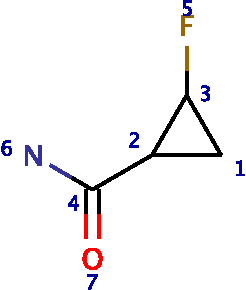
\includegraphics[width=1 true in]{test0-crop}}
    \column{2.8 true in}
    \[
    A = \begin{pmatrix}
0&1&1&0&0&0&0 \\
1&0&1&1&0&0&0 \\
1&1&0&0&1&0&0 \\
0&1&0&0&0&1&1 \\
0&0&1&0&0&0&0 \\
0&0&0&1&0&0&0 \\
0&0&0&1&0&0&0 \\      
    \end{pmatrix}
    \]
  \end{columns}
\end{frame}

\begin{frame}
  \showlogo
  \frametitle{Graph spectrum}
  \framesubtitle{Laplacian}
  Let $D$ be the degree matrix of $G$, i.e., $D_{ii} =
  \text{degree}(v_i)$ and 0 elsewhere, we have the Laplacian $L$
  defined as follows
  \[
  L = D - A,
  \]
  where $A$ is the adjacency matrix.
  \begin{columns}
    \column{1.2 true in}
    \centerline{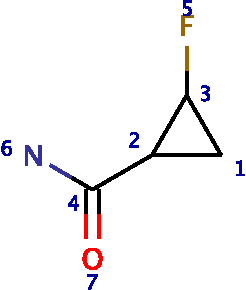
\includegraphics[width=1 true in]{test0-crop}}
    \column{2.8 true in}
    \[
    L = \left(\begin{array}{rrrrrrr}
  2&-1&-1&0&0&0&0 \\
-1&3&-1&-1&0&0&0 \\
-1&-1&3&0&-1&0&0 \\
0&-1&0&3&0&-1&-1 \\
0&0&-1&0&1&0&0 \\
0&0&0&-1&0&1&0 \\
0&0&0&-1&0&0&1 \\
    \end{array}\right)
    \]
  \end{columns}
\end{frame}

\begin{frame}
  \showlogo
  \frametitle{Graph spectrum}
  \framesubtitle{Normalized Laplacian}
  The normalized Laplacian is defined as
  \[
  \tilde L = D^{-\frac{1}{2}}LD^{-\frac{1}{2}},
  \]
  or
  \[
  \tilde L_{ij} = \begin{cases}
    1\quad i = j\\
    -\frac{1}{\sqrt{d_id_j}}\quad i \not= j
  \end{cases}
  \]
  where $d_i$ and $d_j$ are the degrees of $v_i$ and $v_j$,
  respectively.
  \begin{columns}
    \column{1.2 true in}
    \centerline{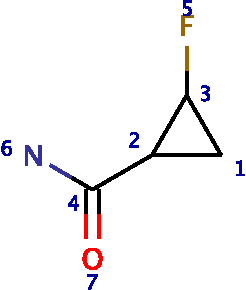
\includegraphics[width=1 true in]{test0-crop}}
    \column{2.8 true in}
    \[
    \tilde L = \tiny\left(\begin{array}{rrrrrrr}
1.0&-0.4&-0.4&0.0&0.0&0.0&0.0 \\
-0.4&1.0&-0.3&-0.3&0.0&0.0&0.0 \\
-0.4&-0.3&1.0&0.0&-0.6&0.0&0.0 \\
0.0&-0.3&0.0&1.0&0.0&-0.6&-0.6 \\
0.0&0.0&-0.6&0.0&1.0&0.0&0.0 \\
0.0&0.0&0.0&-0.6&0.0&1.0&0.0 \\
0.0&0.0&0.0&-0.6&0.0&0.0&1.0 \\      
    \end{array}\right)
    \]
  \end{columns}
\end{frame}

\begin{frame}
  \showlogo
  \frametitle{Spectral properties}
  \begin{itemize}
    \item The spectrum of $A$ is bounded by the maximum degree in $G$,
      i.e., $|\lambda_i| \leq \max_k d(v_k)$ for $k = 1, 2, \ldots,
      n$.  For organic molecules, $|\lambda_i| \leq 4$.
    \item $L$ and $\tilde L$'s spectra are non-negative, i.e., $\lambda_i
      \ge 0$. $L$ and $\tilde L$ are semidefinite.
    \item Multiplicity of $\lambda_i = 0$ in $L$ and $\tilde L$ is the
      number of connected components in $G$. 
    \item The spectrum of $\tilde L$ is bounded by 2, i.e., $0 \le
      \lambda_i \le 2$.
    \item Let $\lambda_1 = 0 \le \lambda_2 \le \cdots \le \lambda_n$ for
      $L$ and $\tilde L$. The first non-zero $\lambda_i$ is the
      \emph{algebraic connectivity} index with the corresponding 
      eigenvector known as the \emph{Fiedler} vector. This vector
      provides near-optimal 2-partition of $G$. The Fiedler vector
      is the foundation of many spectral clustering algorithms.
  \end{itemize}
  \begin{columns}
    \column{1 true in}
    \column{1.2 true in}
    \centerline{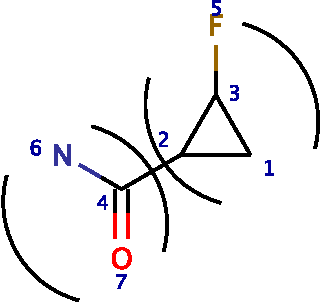
\includegraphics[width=.8 true in]{test0-part-crop}}
    \column{2 true in}
    \[
    \mathbf{v}_2(\tilde L) = \left[\tiny\begin{array}{r}
      0.29255\\
      0.11507\\
      0.44483\\
      -0.53342\\
      0.32870\\
      -0.39416\\
      -0.39416\\
      \end{array}\right]
    \]
    \column{1 true in}
  \end{columns}
\end{frame}

\begin{frame}
  \showlogo
  \frametitle{Spectral hash key}
  \vspace{-1em}
\centerline{$\overbrace{\hbox{\texttt{\color{red}{111ZMSDKX}}}}^{|h_1|=9}\overbrace{\hbox{\texttt{\color{blue}{4LX8LNL6ZR}}}}^{|h_2|=10}\overbrace{\hbox{\texttt{\color{orange}{D728VM5HM7J}}}}^{|h_3|=11}$}
\vspace{-1em}
  \begin{columns}
    \column{5cm}
    \begin{block}{Algorithm}
      \begin{enumerate}[(i)]
      \item Let $\{\lambda_i\}$ be the spectrum of $\tilde L$ (largest component)
      \item $h_1$ is the truncated (45 bits) SHA-1 digest of $\{\lambda_i\}$
      \item $h_2$ is the truncated (50 bits) SHA-1 digest of $h_1$ and \texttt{/c} layer of the largest component
      \item $h_3$ is the truncated (55 bits) SHA-1 digest of $h_2$ and full InChI string
        \item Spectral hash key is an 150-bit string $h_1h_2h_3$
      \end{enumerate}
    \end{block}
    \column{5cm}
    \begin{block}{Properties}
      \begin{itemize}
        \item Hash key is a base-32 encoded string with the alphabet $\{A,\ldots, Z\} \cup \{1,\ldots,9\} \backslash \{E,I,O\}$
        \item Three logical blocks $h_1$, $h_2$, and $h_3$ with progressively increased resolution
          \item Hash chaining allows the individual blocks to be used independently
      \item Structure grouping with sort
      \end{itemize}
    \end{block}
  \end{columns}
\end{frame}

\begin{frame}
  \showlogo
  \frametitle{Spectral hash key by the numbers}
  \framesubtitle{ChEMBL 28}
  \begin{columns}
    \column{7cm}
    \begin{itemize}
    \item 1,268,784 unique values for $h_1$ with   $h_1=\hbox{\texttt{VXL4K9UW2}}$ comprising of 537 structures (peptide)
      \begin{tabular}{ccc}
        \raisebox{-.5\height}{\texttt{WU7MZ9LTZ}} &
        \raisebox{-.5\height}{229} &\raisebox{-.5\height}{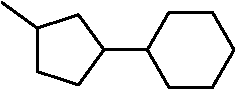
\includegraphics[width=1cm]{WU7MZ9LTZ-crop}}\\
        \raisebox{-.5\height}{\texttt{FHTNW1AYS}} & \raisebox{-.5\height}{234} &\raisebox{-.5\height}{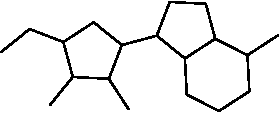
\includegraphics[width=1cm]{FHTNW1AYS-crop}}\\
      \end{tabular}
    \item 1,727,459 unique values for $h_2$ with $h_2 = \hbox{\texttt{9154K6U6NH}}$ comprising of 515 structures
      \begin{tabular}{ccc} \raisebox{-.5\height}{\texttt{72X2TJJJC1}}&\raisebox{-.5\height}{86}&\raisebox{-.5\height}{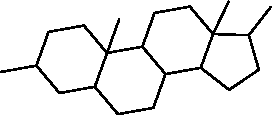
\includegraphics[width=1cm]{3U51T8HJB72X2TJJJC1-crop}}\\
\raisebox{-.5\height}{\texttt{PNNJW7VMJW}}&\raisebox{-.5\height}{79}&\raisebox{-.5\height}{
\includegraphics[width=.5cm]{D2TJDKU9TPNNJW7VMJW-crop}}\\
\raisebox{-.5\height}{\texttt{4B8X9B61KH}}&\raisebox{-.5\height}{70}&\raisebox{-.5\height}{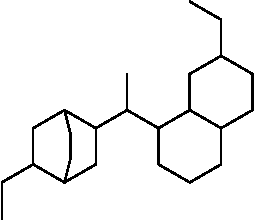
\includegraphics[width=1cm]{PA4F6XKQ44B8X9B61KH-crop}}\\        
      \end{tabular}
    \end{itemize}
    \column{4cm}
    \centerline{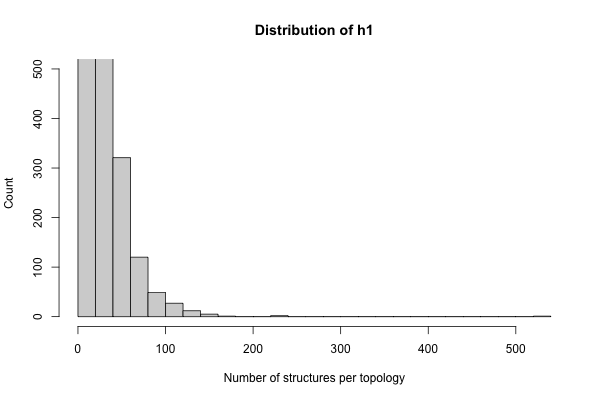
\includegraphics[width=5cm,height=3cm]{h1-dist}}
    \centerline{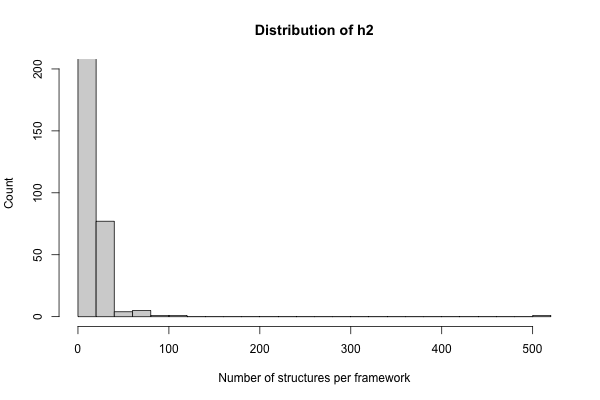
\includegraphics[width=5cm,height=3cm]{h2-dist}}
  \end{columns}
\end{frame}

\begin{frame}
  \showlogoSW  
  \frametitle{Do similar hash keys have similar biological activity?}
  \framesubtitle{Kinase ($h_1$)}
  \begin{columns}
    \column{6cm}
    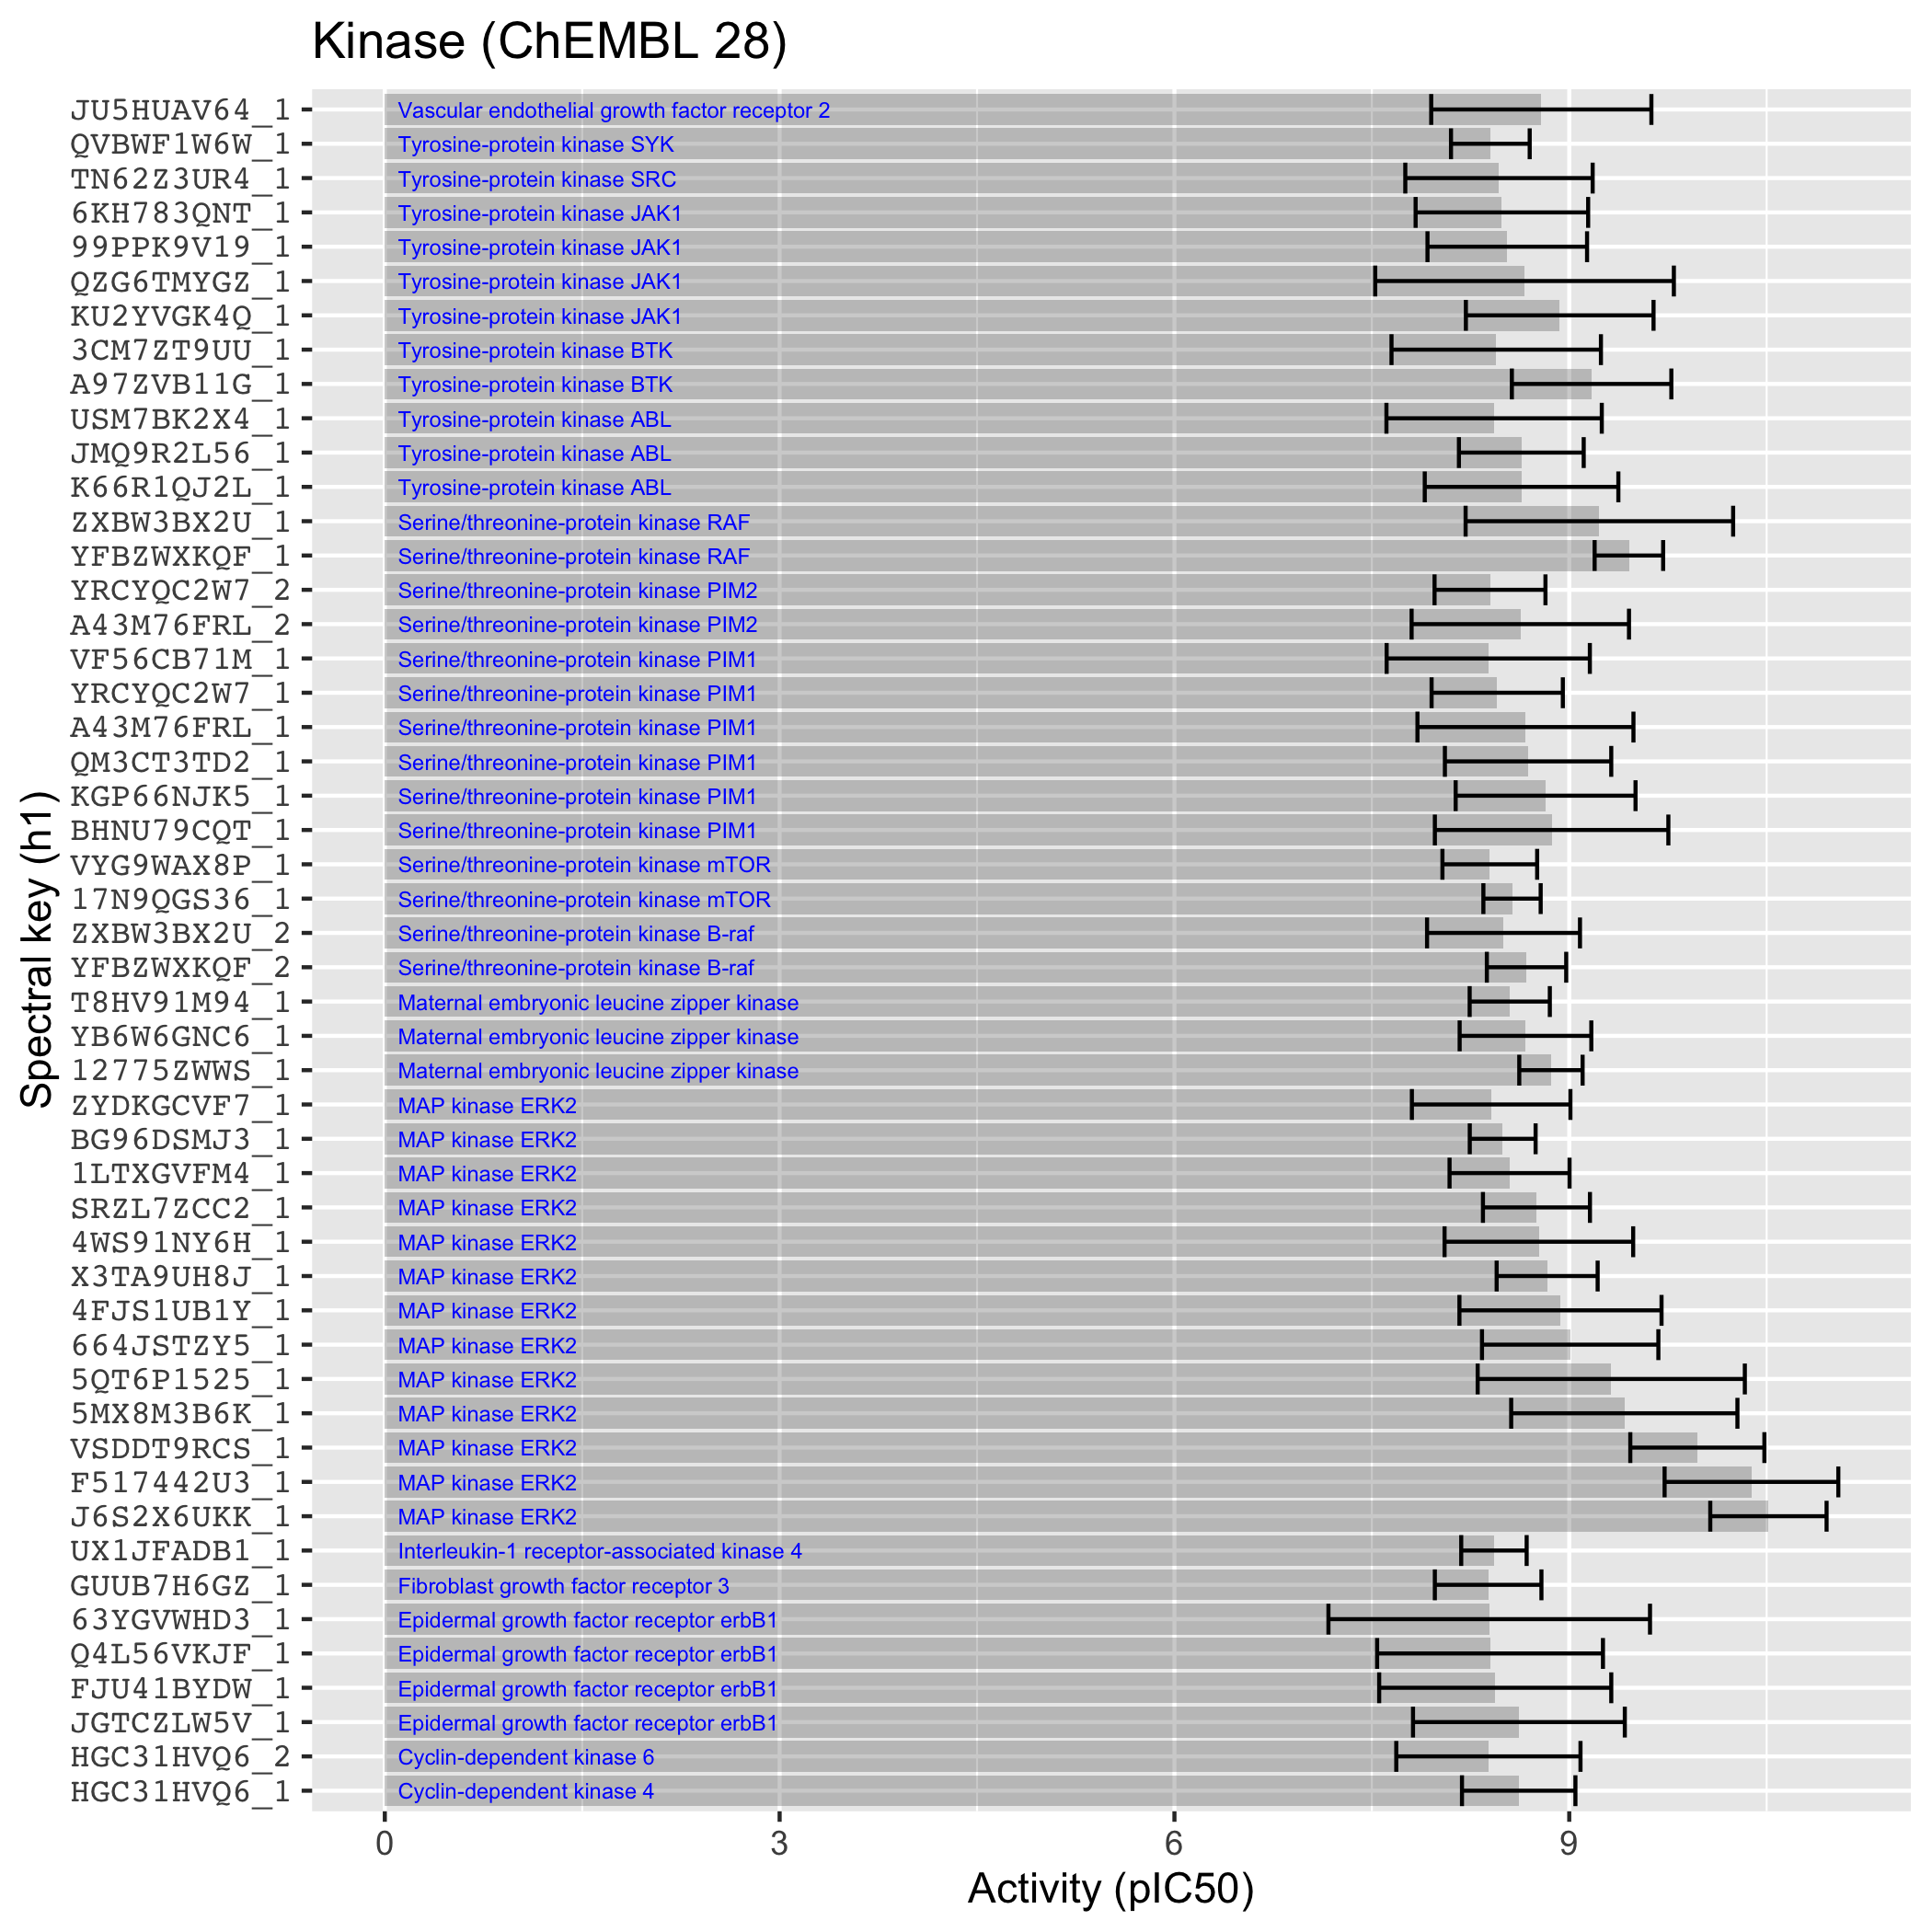
\includegraphics[height=6cm]{spectral_h1_kinase_pIC50}
    \column{6cm}
    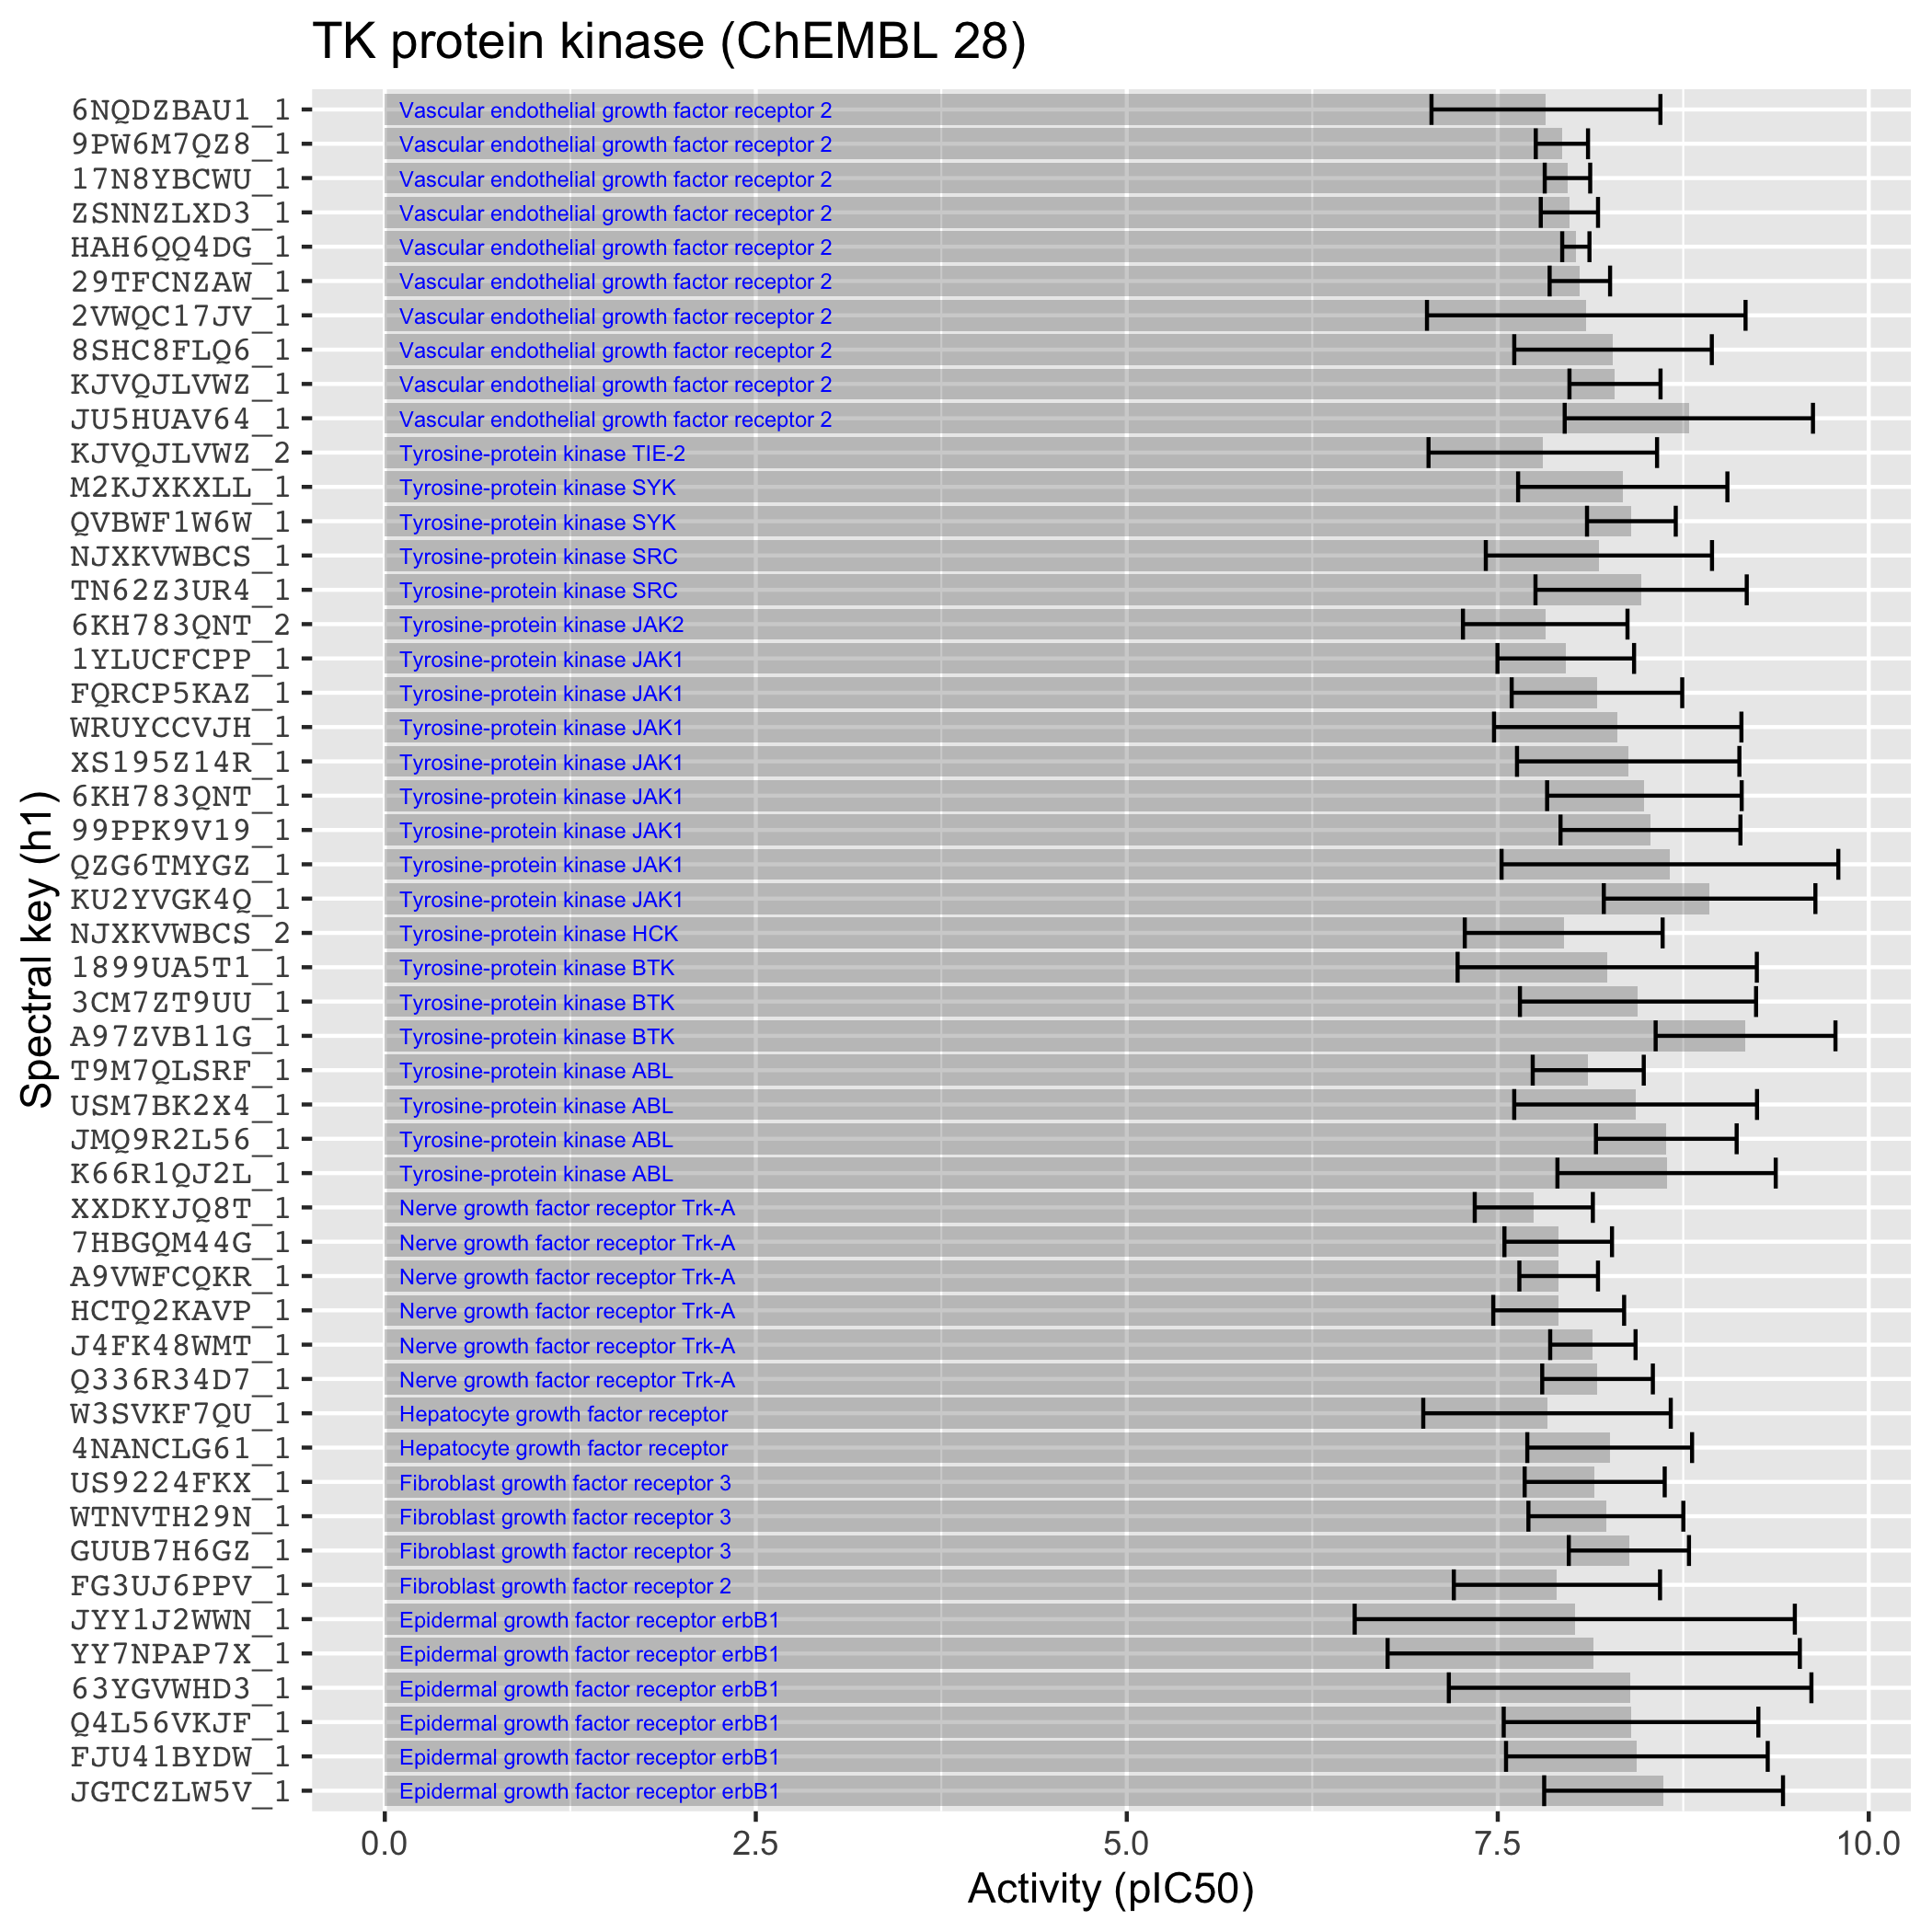
\includegraphics[height=6cm]{spectral_h1_tk_pIC50}
  \end{columns}
\end{frame}
\begin{frame}
  \showlogoSW
  \frametitle{Do similar hash keys have similar biological activity?}
  \framesubtitle{GCPR \& Ion channel ($h_1$)}
  \begin{columns}
    \column{6cm}
    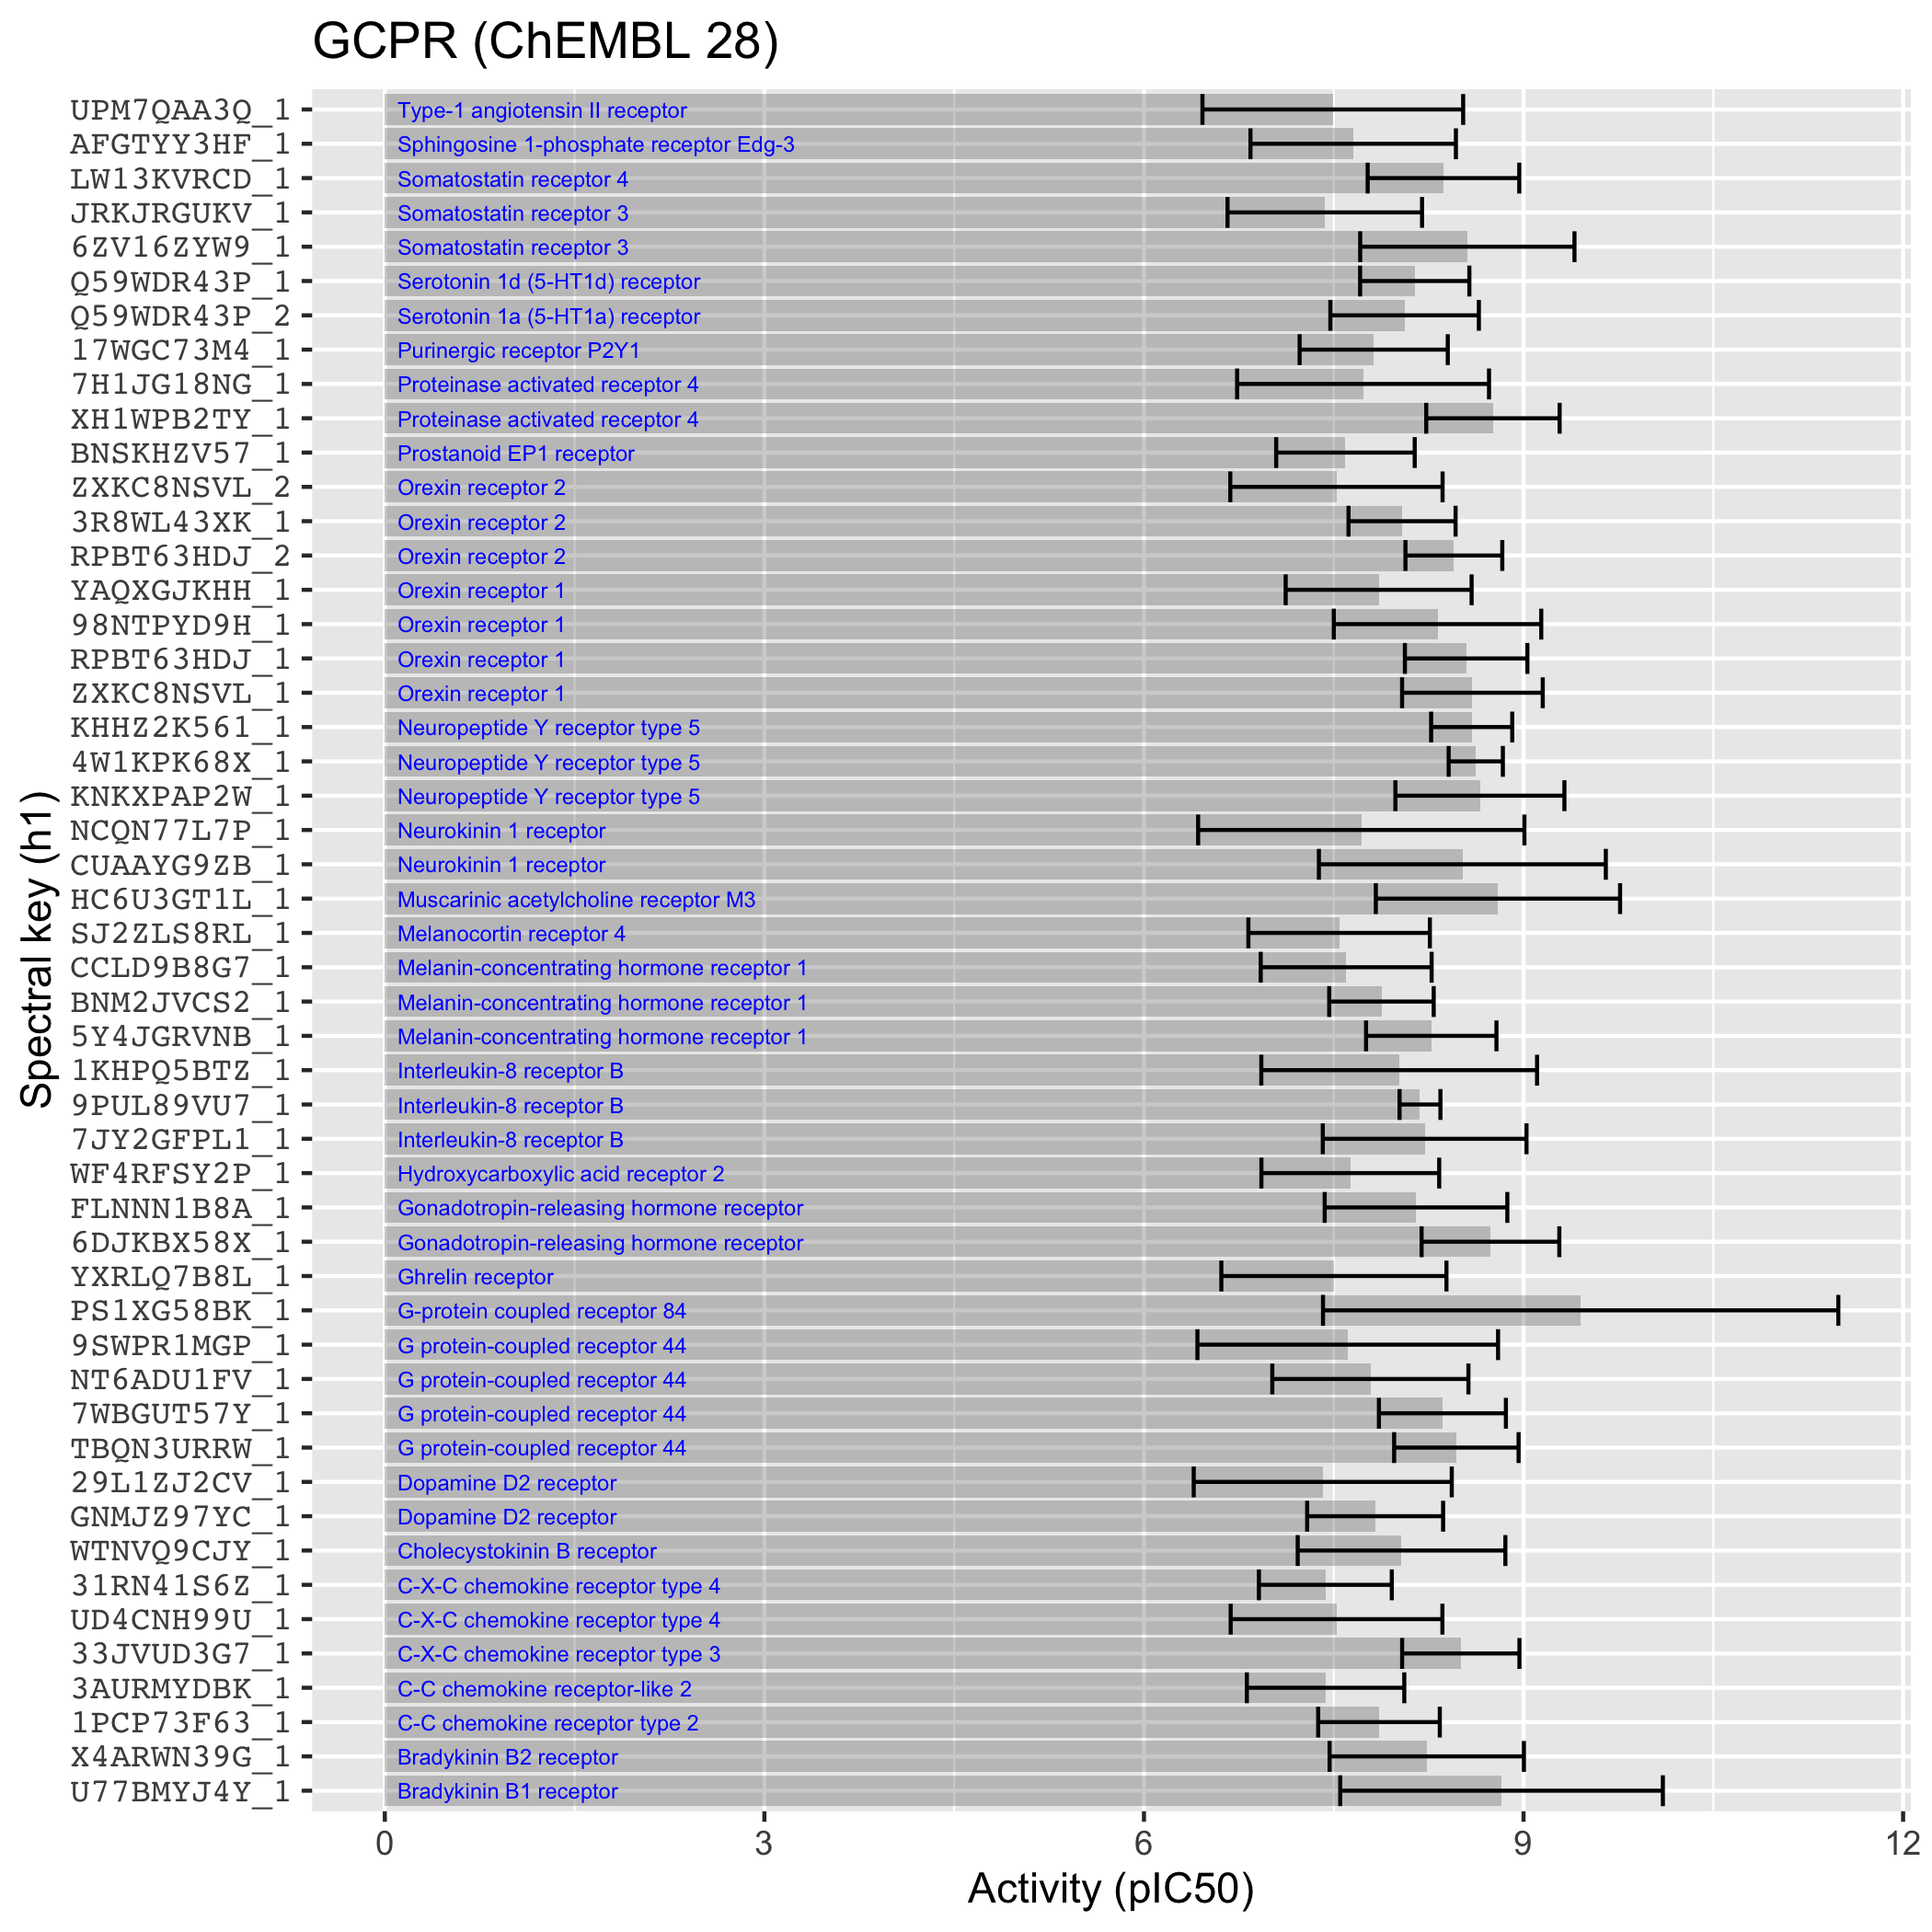
\includegraphics[height=6cm]{spectral_h1_gcpr_pIC50}
    \column{6cm}
    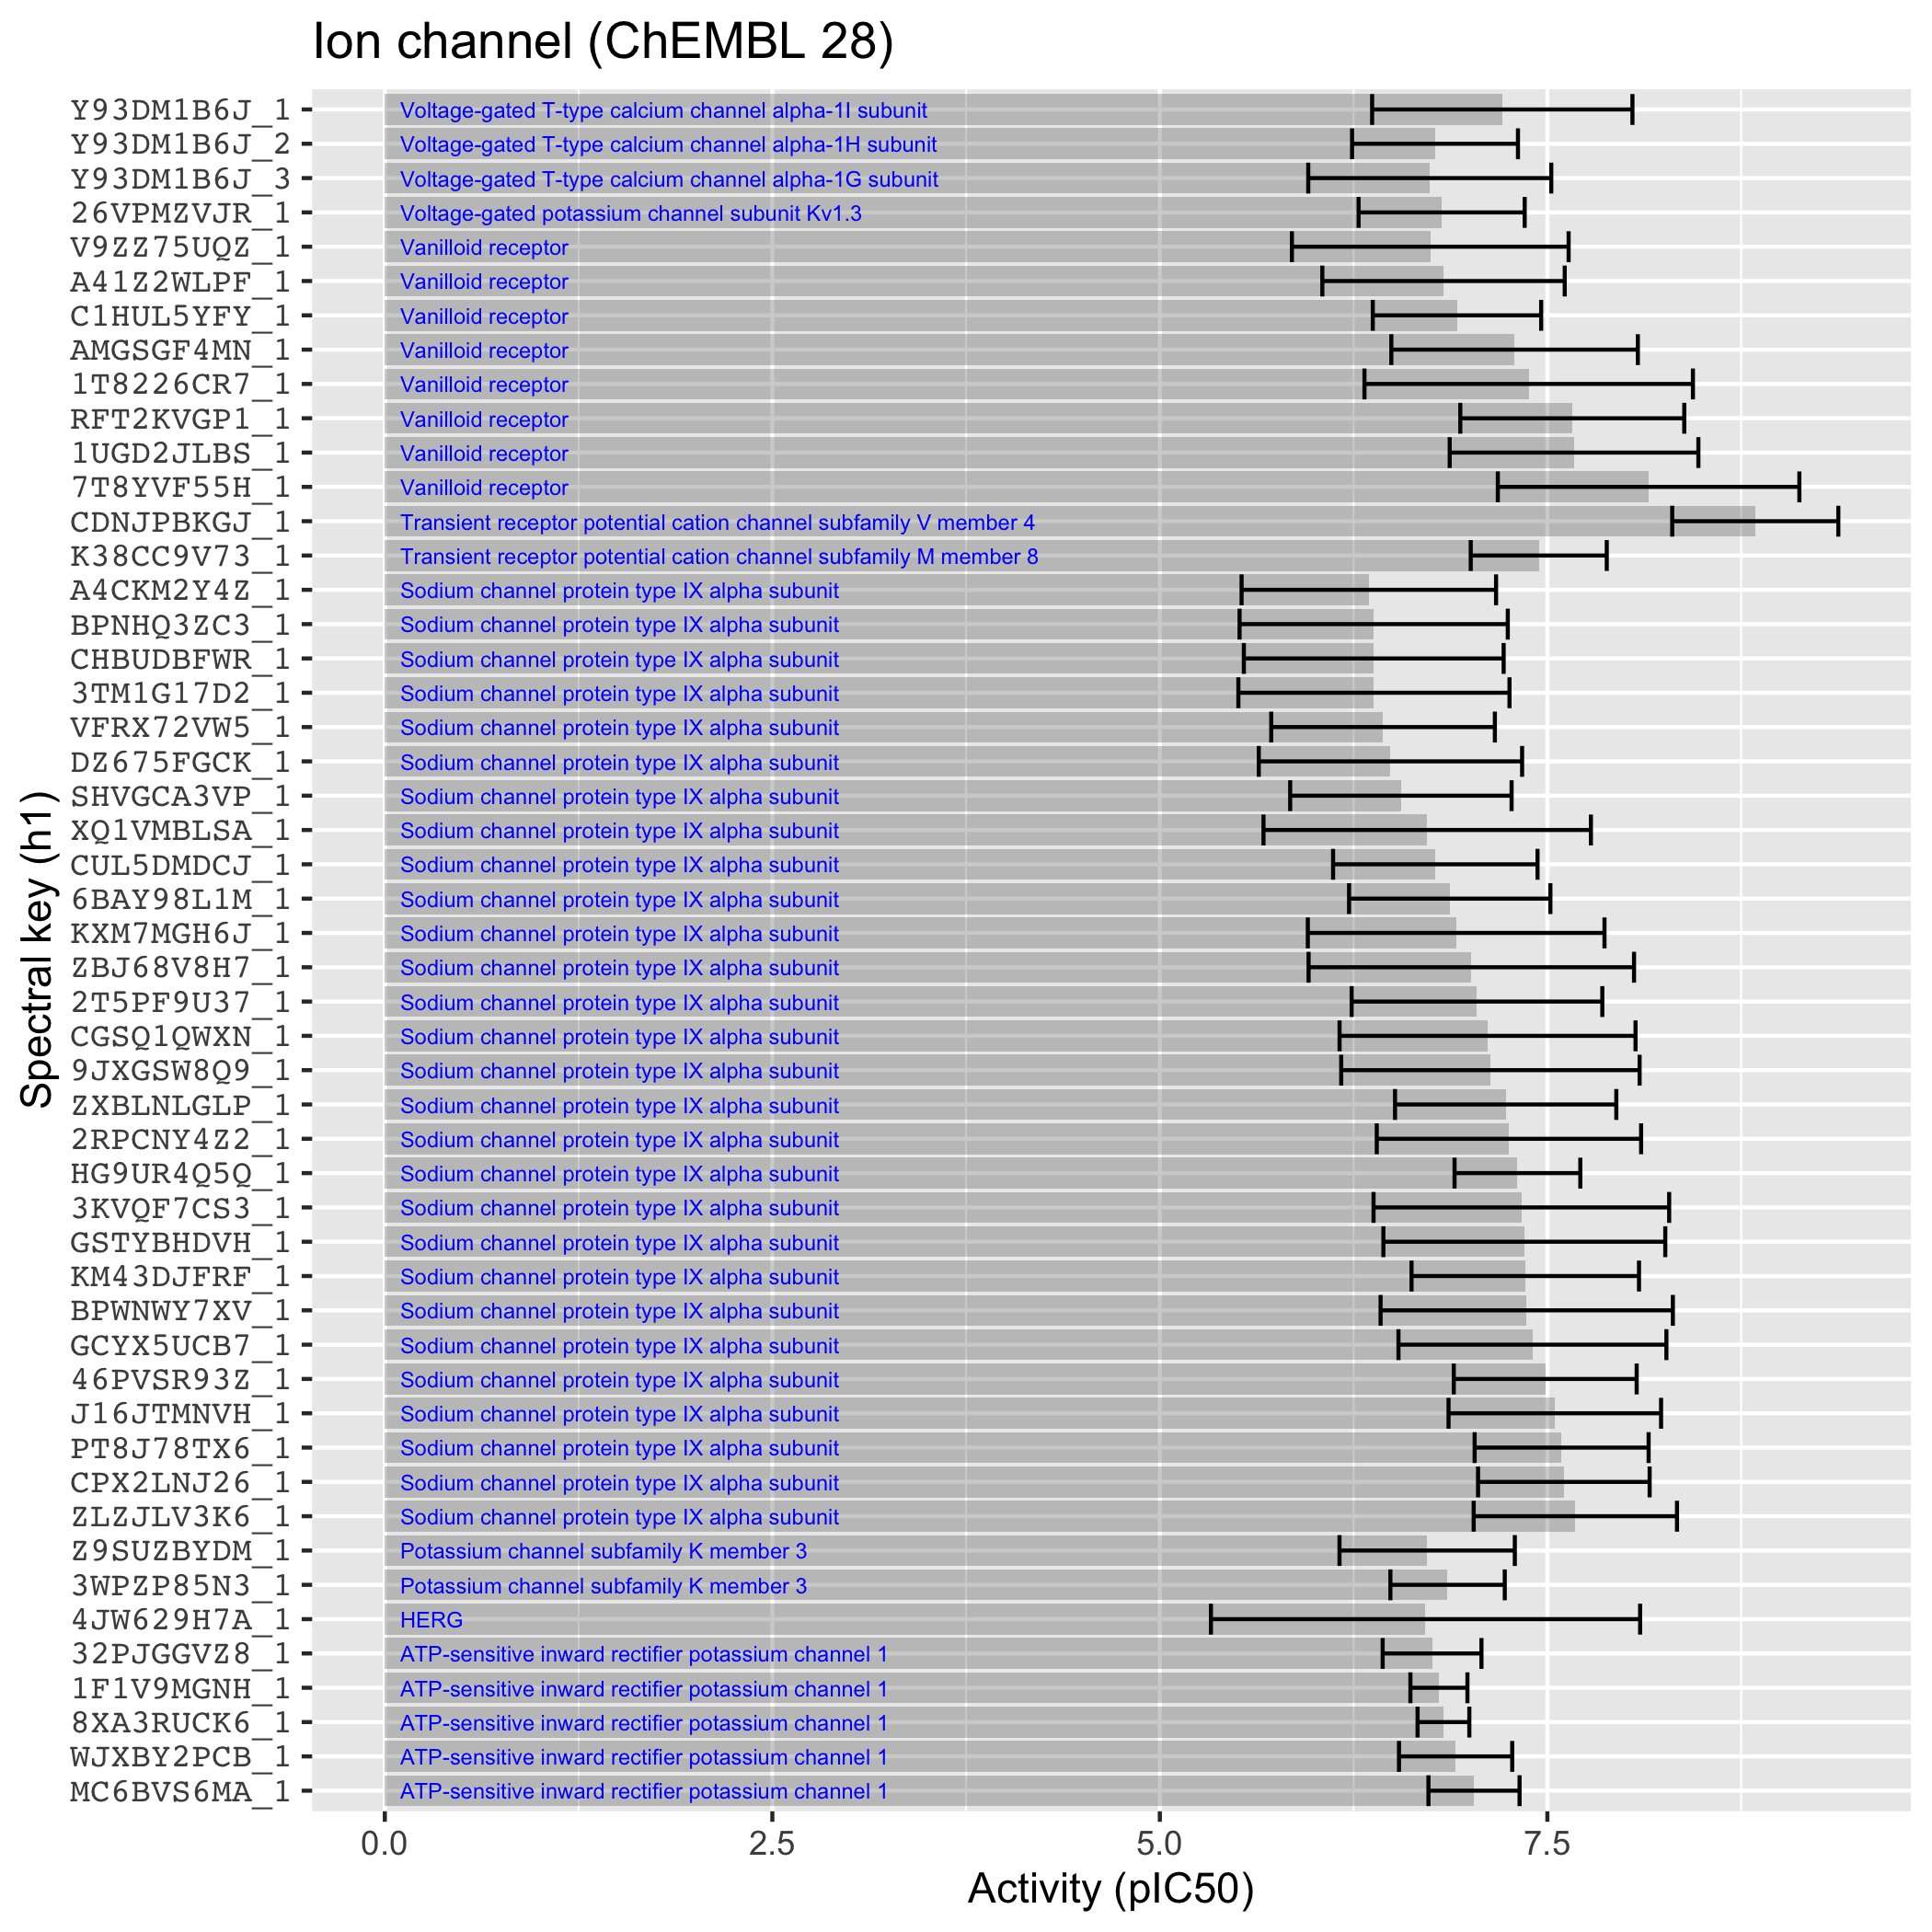
\includegraphics[height=6cm]{spectral_h1_ic_pIC50}
  \end{columns}
\end{frame}

\begin{frame}
  \showlogo
  \frametitle{What is ``similarity''?}
  \framesubtitle{The problem}
  \vspace{-1em}
  \begin{columns}
    \column{7cm}
    What should the similarity be between the following structures? \\ \vspace{1em}
    \centerline{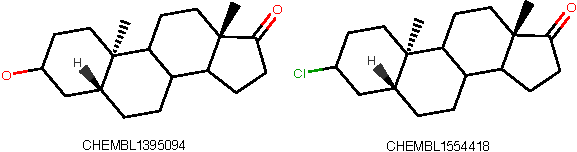
\includegraphics[width=4cm]{CHEMBL1395094-CHEMBL1554418-crop}}
    Tanimoto = 0.55, InChI edit distance = 8
    What about this pair? \\ \vspace{1em}
    \centerline{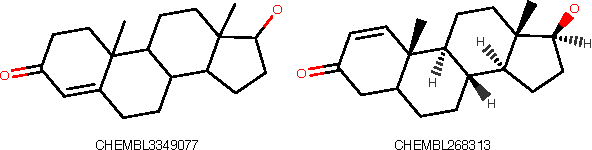
\includegraphics[width=4cm]{CHEMBL3349077-CHEMBL268313-crop}}
    Tanimoto = 1, InChI edit distance = 47

    \color{blue}{\emph{Limitations of the Tanimoto metric are well-recognized within the cheminformatics community, but what about the InChI edit distance?}}
    \column{5cm}
    \begin{tabular}{l}
      \raisebox{-.5\height}{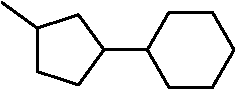
\includegraphics[width=2cm]{WU7MZ9LTZ-crop}}\\
      \raisebox{-.5\height}{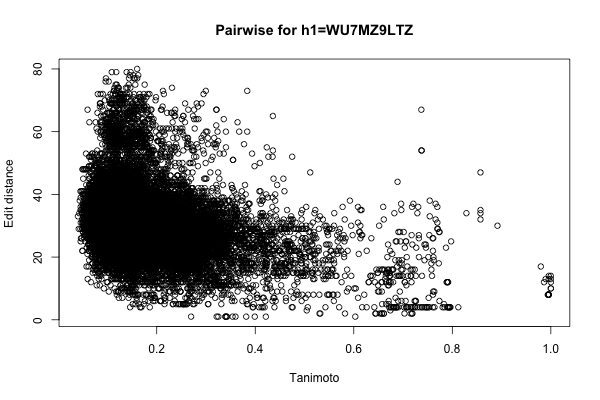
\includegraphics[width=4.5cm]{WU7MZ9LTZ-pairwise}}  \\
      \raisebox{-.5\height}{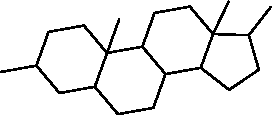
\includegraphics[width=2cm]{3U51T8HJB72X2TJJJC1-crop}}\\     \raisebox{-.5\height}{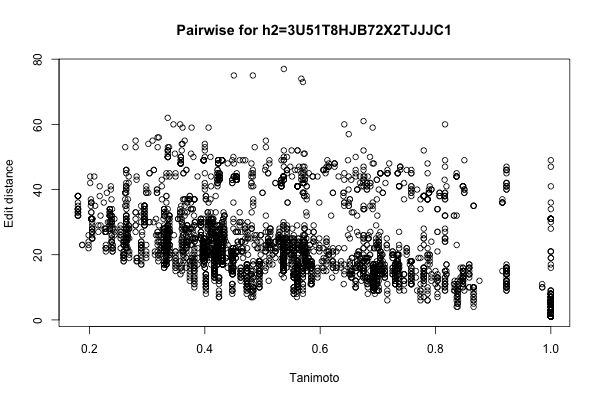
\includegraphics[width=4.5cm]{3U51T8HJB72X2TJJJC1-pairwise}}  \\
    \end{tabular}
  \end{columns}
\end{frame}

\begin{frame}
  \showlogo
  \frametitle{What is ``similarity''?}
  \framesubtitle{What's wrong with InChI edit distance? (a diatribe)}
  \vspace{-1em}
  \begin{itemize}
  \item \emph{Can you translate chemical images to text?}
    \centerline{\texttt{https://www.kaggle.com/c/bms-molecular-translation/}}
  \item Use InChI edit distance as an evaluation metric
  \item Despite our best efforts so far, we're being destroyed by the GPU-bound Python notebook crowds
    \centerline{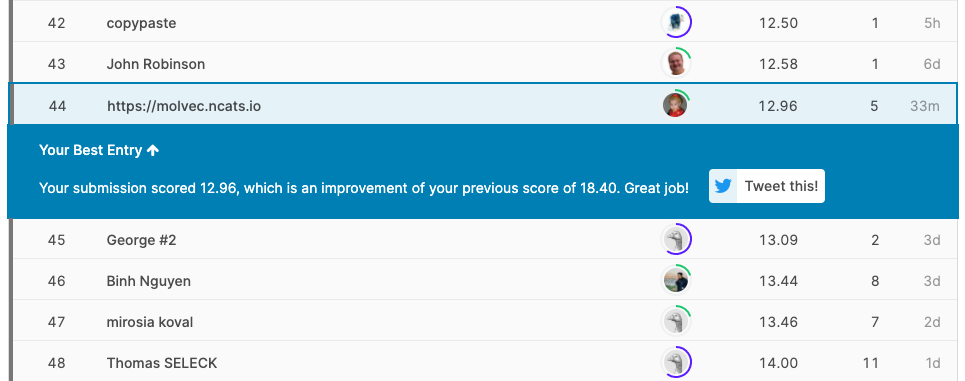
\includegraphics[width=5cm]{molvec-rank}}
  \item Ignorance is bliss (or less is more)
    \begin{center}
      \begin{tabular}{ccc}
        \raisebox{-.5\height}{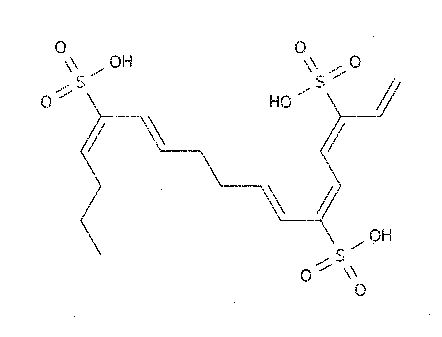
\includegraphics[width=2cm]{bms-image}} &
        \raisebox{-.5\height}{$\rightarrow$} &
        \raisebox{-.5\height}{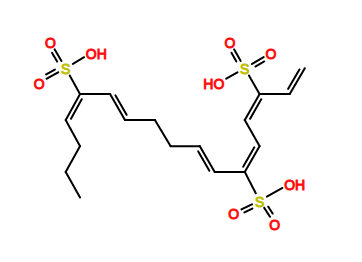
\includegraphics[width=2cm]{molvec-image}}\\
      \end{tabular}
    \end{center}
    Perfect reconstruction, but the extra E/Zs implied by the drawing cost us 34 edit distance!
  \end{itemize}
\end{frame}

\begin{frame}
  \showlogo
  \frametitle{What is ``similarity''?}
  \framesubtitle{Next step}  
  \begin{block}{Challenge to the InChI community}
    \emph{Develop a robust distance or similarity metric for InChI that reflects the chemist's intuitions}
  \end{block}  
  \begin{itemize}
  \item Graph edit distance based on MCS (e.g., NextMove's smallworld)
  \item Edit distance based on graph spectrum
  \end{itemize}
\end{frame}

\begin{frame}
  \showlogo
  \begin{block}{Code availability}
    \begin{itemize}
    \item Self-contained source code in C at
      \centerline{\href{https://github.com/ncats/spectral\_hk}{\texttt{https://github.com/ncats/spectral\_hk}}}
    \item Spectral hash keys generated for ChEMBL 28 are available at
      \centerline{\texttt{mysql -u chembl -h chembl.ncats.io chembl28\_ncats}}
    \item Welcome questions and feedback: \texttt{nguyenda@mail.nih.gov}
    \end{itemize}
  \end{block}
  \begin{block}{Acknowledgements}
    \begin{itemize}
    \item Alexey Zakharov
    \item Tyler Peryea (FDA)
    \item Lu Chen
    \item Ewy Math\'e
    \item Noel Southall
    \end{itemize}
  \end{block}
  \begin{block}{Funding}
    NCATS intramural
  \end{block}
\end{frame}

\end{document}
